\documentclass[12pt]{article}

\usepackage{fancyhdr}
\usepackage{amsmath}
\usepackage{graphicx}
\usepackage[hidelinks]{hyperref}
\usepackage[T1]{fontenc}
\usepackage[frenchb]{babel}
\usepackage[utf8]{inputenc}
\usepackage{moresize}
\usepackage{color, colortbl}
\usepackage{lastpage}
\usepackage[
top    = 1cm,
bottom = 4cm,
left   = 2.50cm,
right  = 2.50cm]{geometry}

\definecolor{Gray}{gray}{0.9}

\usepackage{subfiles}


\pagestyle{fancy}
\setlength{\headheight}{70pt}
\renewcommand\headrulewidth{1pt}

\documentclass[../main.tex]{subfiles}
\graphicspath{{assets/}{../assets/}}

\begin{document}

    

\end{document}

\begin{document}
\begin{titlepage}
    \begin{center}
        
\includegraphics[scale=1]{./assets/logo_omniware.PNG}
        \vfill
        \Huge
        Dossier de Spécification

        \HUGE
        \textbf{Moteur de Recherche}
        \vfill
        \normalsize
        \textbf{Destinataire : }\\ 
        Julien PINQUIER\\
        \vspace{1cm}
        \textbf{Auteurs : }\\ 
        Nelson SANCHEZ\\ 
        Guillaume ROUSSIN\\ 
        Constant ROUX\\ 
        Peter PIRIOU--DEZY\\
        Julian TRANI\par
        \vfill
        
\includegraphics[scale=0.5]{./assets/logo_ut3.jpg}
    \end{center}
\end{titlepage}
\begin{titlepage}
\end{titlepage}

\newpage

\section{Suivi du document}
\vspace{0.5cm}
\begin{center}
    \begin{tabular}{|c|c|c|}
        \hline
        \rowcolor{Gray}Version & Date & Objet de la mise à jour \\
        \hline
        1.0 & 03/11/2021 & Création du document \\
        1.1 & 05/11/2021 & Correctifs suite à la réunion client \\
        1.2 & 08/11/2021 & Correctifs suite aux remarques client \\
        \hline
      \end{tabular}
\end{center}

\newpage
\tableofcontents
\listoffigures
\newpage

\documentclass[../main.tex]{subfiles}
\graphicspath{{assets/}{../assets/}}

\begin{document}

    \section{Contexte}
    \subsection{Description entreprise}
    \paragraph{}
    \textbf{OmniWare} est une \textbf{entreprise française} spécialisée dans la conception et le développement de \textbf{logiciels informatiques} pour les secteurs de l’\textbf{aéronautique}, du \textbf{spatial}, de l’\textbf{automobile} et, plus généralement, de la \textbf{robotique}. En 2019, elle réalisait un chiffre d’affaires d’environ \textbf{45 millions d’euros} et employait plus \textbf{350 employés} dans plusieurs établissements dont le principal se situe à \textbf{Toulouse}. La société est devenue en 2020 une filiale de la société japonaise \textbf{ZMP} dont le siège social est à Tokyo.
    \subsection{Objectif}
    \paragraph{}
    De nos jours, l’accès à l’information est un enjeu essentiel. Il faut donc pouvoir accéder à une grande quantité de documents mis à disposition (Internet, archives…) à l’aide d’une description synthétique de leurs contenus. Pour cela, nous devrons passer d’abord par une phase d’indexation automatique.

    \paragraph{}
    Les documents traités seront de nature diverse et seront enregistrés dans un format standard prédéfini. La description synthétique d’un document se basera sur sa nature et son contenu. Cette description sera ensuite utilisée par un moteur de recherche.

    \paragraph{}
    L’utilisateur ne connaît pas le fonctionnement du moteur de recherche, ni la méthode d’indexation des données, le logiciel doit être simple d’utilisation. Toute la phase de configurations, paramétrages et méthodes est gérée par les administrateurs.

\end{document}
\newpage

\documentclass[../main.tex]{subfiles}
\graphicspath{{assets/}{../assets/}}

\begin{document}
    
    \section{Description détaillée du logiciel}
    \subsection{Interfaces (entrées/sorties)}
    \paragraph{}
    Afin de permettre l'interaction entre l’utilisateur et l’application, nous allons utiliser le clavier et la souris comme entrées du programme. Cette communication sera appelée interface et sera constituée uniquement de menus textuels.

    \paragraph{}
    Voici un schéma qui représente les différentes interactions du programme avec son environnement:

    \begin{figure}[h]
        \begin{center}
            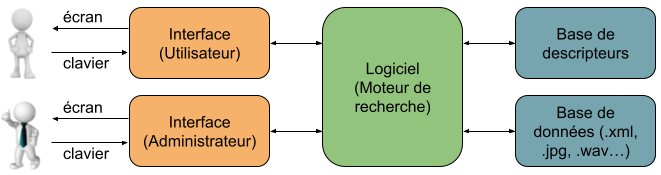
\includegraphics[scale=0.6]{assets/diagrams/pfr_entrees_sorties.png}
            \caption{Diagramme des interfaces de l'application}
        \end{center}
    \end{figure}

    \subsection{Fonctionnalités}
    \subsubsection{Indexation}
    \paragraph{}
    Elle consiste à créer un descripteur de fichier selon le type de document ajouté et les paramètres (modifiables par un administrateur). Il sera ensuite ajouté dans la base de descripteurs qui contient tous les descripteurs disponibles. Cette base sera sauvegardée dans un fichier textuel suivant le prototype suivant:
    \paragraph{}
    \noindent L’indexation change en fonction du type de recherche:
    \begin{itemize}
        \item \underline{Texte}: Une méthode de base consiste à repérer la présence de mots clés et leur nombre d'occurrences. Nous retrouverons une fonction de nettoyage pour enlever les balises et une fonction de filtrage pour retirer les mots outils.
        \item \underline{Image}: Le but est de représenter synthétiquement le contenu de l’image. Nous retrouverons une fonction de quantification afin de limiter les calculs et une fonction d’histogramme.
        \item \underline{Audio}: Une méthode simple consiste à découper le signal en plusieurs fenêtres de taille n échantillons puis de calculer pour chacune de celles-ci un histogramme composé de m intervalles. On aura donc une fonction d’histogramme.
    \end{itemize}

    \subsubsection{Comparaison}
    \paragraph{}
    Une fois l’indexation réalisée nous pouvons réaliser la comparaison de documents par l'intermédiaire des descripteurs de fichier. Pour que les documents soient identiques, il faut que les deux descripteurs soient strictement les mêmes. Sinon, nous parlerons de similarité selon un certain pourcentage de similitude (aussi appelé taux de confiance), pour cela, un calcul de distance sera effectué. Dans notre, il sera possible d’utiliser une fonction générique fonctionnant pour tous types de descripteurs.

    \subsubsection{Moteur de recherche}
    \paragraph{}
    L’utilisateur, depuis le moteur de recherche, doit d’abord choisir le type de recherche qu’il veut faire:
    \begin{itemize}
        \item recherche Texte: il pourra donner soit un mot-clef, soit le chemin vers un fichier texte.
        \item recherche Image: il aura la possibilité d’entrer une couleur (en choisissant une couleur dans une palette prédéfinie ou bien en donnant la couleur exacte par code hexa), une image RGB ou une image en niveaux de gris.
        \item recherche Audio: il devra donner un fichier audio en entrée.
    \end{itemize}

    \paragraph{}
    À la suite de la requête sur l’application, le logiciel renvoie à l’utilisateur la liste des documents trouvés, allant de celui avec la plus forte similitude avec la recherche jusqu’à celui ayant la moins forte. Si le pourcentage de similitude est inférieur à 5\% alors rien ne sera affiché. Les documents trouvés ainsi que leurs descripteurs pourront être consultables par l’utilisateur. Le document ayant le taux de confiance le plus élevé sera ouvert automatiquement (ouvert dans un éditeur de texte pour la recherche Texte, dans un visionneur d’images pour la recherche Image et la zone audio possédant la similarité la plus proche dans un lecteur audio pour la recherche Audio).

    \paragraph{}
    De plus, seront présentes différentes vérifications:
    \begin{itemize}
        \item vérification de la saisie clavier,
        \item vérification de l’indexation des documents,
        \item vérification des chemins d’accès aux fichiers,
        \item vérification des types passés en paramètres.
    \end{itemize}

    \paragraph{}
    En cas d’erreur lors de la vérification, un message sera affiché à l’utilisateur et une solution proposée pour continuer l’utilisation du logiciel. (Exemple: si le chemin d’un fichier est inexistant, l’application propose d’entrer à nouveau le chemin).

    \paragraph{}
    Voici un diagramme de séquence assez généraliste de l’exécution du moteur de recherche depuis le mode utilisateur:

    \paragraph{}
    Voici un diagramme de séquence assez généraliste de processus d’indexation de fichier:

    \subsection{Scénario}
    \paragraph{}
    Voici une exécution de l’application du point de vue de l’utilisateur, dans ce scénario, nous voulons parmi les images, rechercher par code couleur. Ensuite, il affiche les résultats dans la console puis demande à l'utilisateur de choisir sa visualisation.

    \begin{figure}[h]
        % \input{assets/use_cases/user.txt}
        \centering
        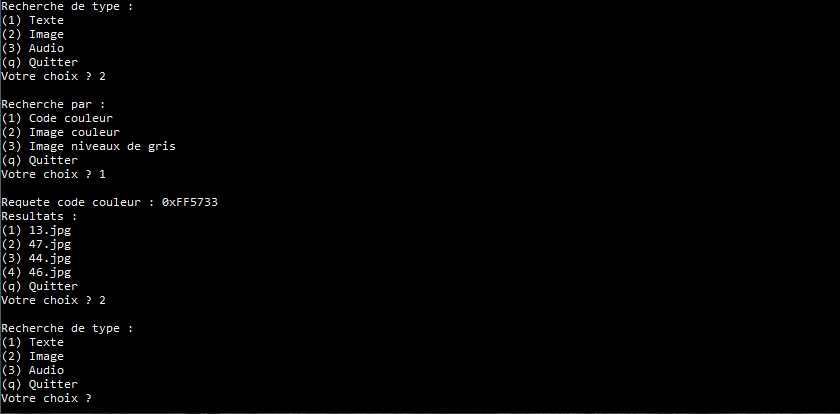
\includegraphics[width=160mm]{use_cases/scenario utilisateur.PNG}
        \caption{scénario enviseageable pour un utilisateur}
    \end{figure}

\end{document}
\newpage

\documentclass[../main.tex]{subfiles}
\graphicspath{{assets/}{../assets/}}

\begin{document}

    \section{Prévision d'organisation du projet}


    \paragraph{}
    Le code source de l’application sera disponible sur Github à l’adresse suivante: \url{https://github.com/Guillaume-prog/projet-fil-rouge}

    \paragraph{}
    Au sein de l’équipe, des outils de gestion comme Trello vont être utilisés.

    \subsection{Déroulement prévu}

    \paragraph{}
    Voici une planification prévisionnelle du projet sous la forme d’un diagramme de Gantt réalisé avec Gantt Project:

    \begin{figure}[H]
        \centering
        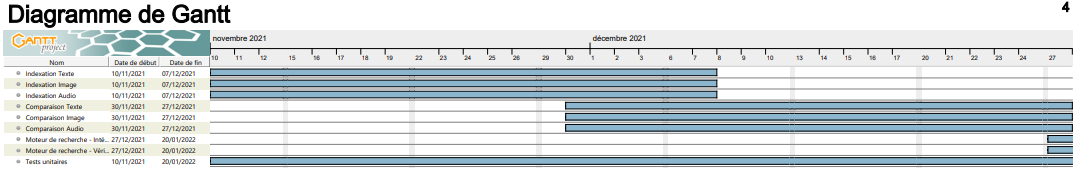
\includegraphics[width=160mm]{gantt/gantt_calendar.png}
        \caption{Diagramme de Gantt du projet}
    \end{figure}

    \begin{figure}[H]
        \centering
        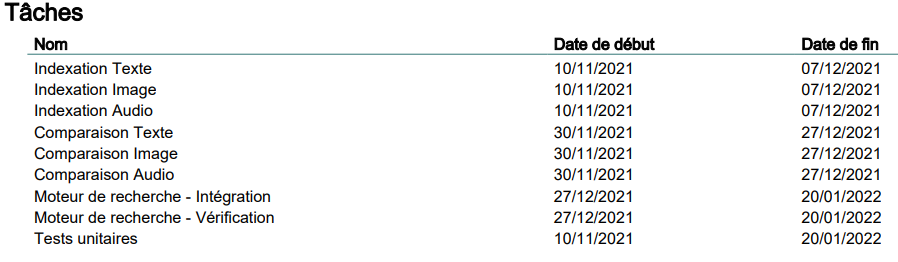
\includegraphics[width=160mm]{gantt/gantt_list.png}
        \caption{Tableau récapitulatif des tâches à réaliser issu du diagramme de Gantt}
    \end{figure}

    \subsection{Répartition des tâches}

    \begin{table}[H]
        \centering
        \begin{tabular}{ | m{10em} | m{10em} | m{10em} | }
            \hline
            \rowcolor{Gray} Tâches & Sous-tâches & Affectation des tâches \\
            \hline
            \multirow{3}{10em}{Indexation} 
            & Indexation texte & Guillaume \& Peter \\
            \cline{2-3}
            & Indexation image & Constant \& Peter \\
            \cline{2-3}
            & Indexation audio & Julian \& Nelson \\
            \hline

            \multirow{3}{10em}{Comparaison} 
            & Comparaison texte & Guillaume \& Constant \\
            \cline{2-3}
            & Comparaison image & Constant \& Peter \\
            \cline{2-3}
            & Comparaison audio & Julian \& Nelson \\
            \hline

            \multirow{2}{10em}{Moteur de recherche} 
            & Intégration & Toute l'équipe \\
            \cline{2-3}
            & Vérifications & Julian \& Nelson \\
            \hline

            \multirow{1}{10em}{Test} & / & Toute l'équipe \\
            \hline


            \hline
        \end{tabular}
        \caption{Récapitulatif des affectations des tâches du projet}
    \end{table}

\end{document}
\newpage

\section{Glossaire}
\paragraph{Balise}
Une balise est un nom commode pour désigner les constructions entre deux chevrons (<, >) dans un fichier XML. Nous distinguons globalement les balises ouvrantes <élément attribut="valeur"> et les balises fermantes </élément> (sans attributs et commençant par une barre oblique).

\paragraph{Token}
Un token est une chaîne de caractères finissant par '\textbackslash 0' en langage C. Un texte est une suite de tokens séparés par des espaces. Nous considérons qu’un token a une taille maximale. Seuls les tokens correspondant à des mots pertinents seront retenus.

\paragraph{Descripteur}
Représentation synthétique d’un document par diverses informations. Elle varie selon le type du document et les paramètres choisis par l’administrateur.

\paragraph{Interface}
Dispositif qui permet la communication entre un utilisateur et le logiciel.
\newpage

\end{document}